\documentclass[11pt, aspectratio=169]{beamer}
\usetheme[progressbar=frametitle, block=fill]{metropolis}

\usepackage[utf8]{inputenc}
\usepackage{tikz}
\usetikzlibrary{trees, shapes.geometric, arrows.meta, positioning, calc, fit, backgrounds}
\usepackage{booktabs}
\usepackage{graphicx}
\usepackage{xcolor}
\usepackage{colortbl}

\definecolor{primary}{RGB}{35, 55, 59}
\definecolor{accent}{RGB}{235, 129, 27}
\definecolor{success}{RGB}{20, 176, 61}
\definecolor{nodebg}{RGB}{190, 195, 200}
\definecolor{labelgreen}{RGB}{0, 100, 0}

\tikzset{
    hnode/.style={circle, draw=primary, thick, fill=white, minimum size=0.6cm, inner sep=0pt, font=\small},
    hl/.style={thick, primary},
    highlight/.style={circle, draw=accent, thick, fill=accent!10, minimum size=0.6cm, inner sep=0pt, font=\small},
    bhnode/.style={circle, draw=black, thick, fill=nodebg, minimum size=0.65cm, inner sep=0pt, font=\small\bfseries},
    rootlink/.style={dotted, thick, black},
    treelink/.style={solid, thick, black},
    bh/.style={circle, draw=black, thick, fill=nodebg, minimum size=0.45cm, inner sep=0pt, font=\bfseries\sffamily\tiny},
    bhb/.style={circle, draw=black, thick, fill=blue!80!black, text=white, minimum size=0.45cm, inner sep=0pt, font=\bfseries\sffamily\tiny},
    bhr/.style={circle, draw=black, thick, fill=red!70!black, text=white, minimum size=0.45cm, inner sep=0pt, font=\bfseries\sffamily\tiny},
    lnk/.style={thick, black},
    dlnk/.style={thick, black, densely dotted}
}

\newcommand{\treeSix}[3]{
    \begin{scope}[shift={(#1,#2)}, every node/.style={#3}]
        \node (n6) at (0,0) {6}; \node (n44) at (0,-1) {44};
        \node (n10) at (-1,-1) {10}; \node (n17) at (-1,-2) {17};
        \node (n29) at (-2,-1) {29}; \node (n31) at (-2,-2) {31}; \node (n48) at (-3,-2) {48}; \node (n50) at (-3,-3) {50};
        \node (n8) at (-4,-1) {8}; \node (n22) at (-4,-2) {22}; \node (n23) at (-5,-2) {23}; \node (n24) at (-5,-3) {24};
        \node (n30) at (-6,-2) {30}; \node (n32) at (-6,-3) {32}; \node (n45) at (-7,-3) {45}; \node (n55) at (-7,-4) {55};
        \draw[lnk] (n6)--(n44); \draw[lnk] (n6)--(n10); \draw[lnk] (n10)--(n17);
        \draw[lnk] (n6)--(n29); \draw[lnk] (n29)--(n31); \draw[lnk] (n29)--(n48); \draw[lnk] (n48)--(n50);
        \draw[lnk] (n6)--(n8); \draw[lnk] (n8)--(n22); \draw[lnk] (n8)--(n23); \draw[lnk] (n23)--(n24);
        \draw[lnk] (n8)--(n30); \draw[lnk] (n30)--(n32); \draw[lnk] (n30)--(n45); \draw[lnk] (n45)--(n55);
    \end{scope}
}
\newcommand{\treeBZero}[3]{
    \begin{scope}[shift={(#1,#2)}, every node/.style={#3}]
        \node (n1) at (0,0) {1};
    \end{scope}
}
\newcommand{\treeBOne}[3]{
    \begin{scope}[shift={(#1,#2)}, every node/.style={#3}]
        \node (n1) at (0,0) {1}; \node (n2) at (0,-1) {2}; \draw[lnk] (n1)--(n2);
    \end{scope}
}
\newcommand{\treeBTwo}[3]{
    \begin{scope}[shift={(#1,#2)}, every node/.style={#3}]
        \node (n1) at (0,0) {1}; \node (n3) at (0,-1) {3};
        \node (n2) at (-1,-1) {2}; \node (n4) at (-1,-2) {4};
        \draw[lnk] (n1)--(n3); \draw[lnk] (n1)--(n2); \draw[lnk] (n2)--(n4);
    \end{scope}
}
\newcommand{\treeBThree}[3]{
    \begin{scope}[shift={(#1,#2)}, every node/.style={#3}]
        \node (n1) at (0,0) {1}; \node (n5) at (0,-1) {5};
        \node (n3) at (-1,-1) {3}; \node (n7) at (-1,-2) {7};
        \node (n2) at (-2,-1) {2}; \node (n6) at (-2,-2) {6}; 
        \node (n4) at (-3,-2) {4}; \node (n8) at (-3,-3) {8};
        \draw[lnk] (n1)--(n5); \draw[lnk] (n1)--(n3); \draw[lnk] (n3)--(n7);
        \draw[lnk] (n1)--(n2); \draw[lnk] (n2)--(n6); \draw[lnk] (n2)--(n4); \draw[lnk] (n4)--(n8);
    \end{scope}
}
\newcommand{\treeThree}[3]{
    \begin{scope}[shift={(#1,#2)}, every node/.style={#3}]
        \node (n3) at (0,0) {3}; \node (n37) at (0,-1) {37}; \draw[lnk] (n3)--(n37);
    \end{scope}
}
\newcommand{\treeEighteen}[3]{
    \begin{scope}[shift={(#1,#2)}, every node/.style={#3}]
        \node (n18) at (0,0) {18};
    \end{scope}
}
\newcommand{\treeFifteen}[3]{
    \begin{scope}[shift={(#1,#2)}, every node/.style={#3}]
        \node (n15) at (0,0) {15}; \node (n33) at (0,-1) {33};
        \node (n28) at (-1,-1) {28}; \node (n41) at (-1,-2) {41};
        \draw[lnk] (n15)--(n33); \draw[lnk] (n15)--(n28); \draw[lnk] (n28)--(n41);
    \end{scope}
}
\newcommand{\treeSeven}[3]{
    \begin{scope}[shift={(#1,#2)}, every node/.style={#3}]
        \node (n7) at (0,0) {7}; \node (n25) at (0,-1) {25}; \draw[lnk] (n7)--(n25);
    \end{scope}
}
\newcommand{\treeTwelve}[3]{
    \begin{scope}[shift={(#1,#2)}, every node/.style={#3}]
        \node (n12) at (0,0) {12};
    \end{scope}
}
\newcommand{\treeTwelveMerged}[3]{
    \begin{scope}[shift={(#1,#2)}, every node/.style={#3}]
        \node (n12) at (0,0) {12}; \node (n18) at (0,-1) {18}; \draw[lnk] (n12)--(n18);
    \end{scope}
}
\newcommand{\treeThreeMerged}[3]{
    \begin{scope}[shift={(#1,#2)}, every node/.style={#3}]
        \node (n3) at (0,0) {3}; \node (n37) at (0,-1) {37};
        \node (n7) at (-1,-1) {7}; \node (n25) at (-1,-2) {25};
        \draw[lnk] (n3)--(n37); \draw[lnk] (n3)--(n7); \draw[lnk] (n7)--(n25);
    \end{scope}
}
\newcommand{\treeThreeFinal}[3]{
    \begin{scope}[shift={(#1,#2)}, every node/.style={#3}]
        \node (n3) at (0,0) {3}; \node (n37) at (0,-1) {37};
        \node (n7) at (-1,-1) {7}; \node (n25) at (-1,-2) {25};
        \node (n15) at (-2,-1) {15}; \node (n33) at (-2,-2) {33};
        \node (n28) at (-3,-2) {28}; \node (n41) at (-3,-3) {41};
        \draw[lnk] (n3)--(n37); \draw[lnk] (n3)--(n7); \draw[lnk] (n7)--(n25);
        \draw[lnk] (n3)--(n15); \draw[lnk] (n15)--(n33); \draw[lnk] (n15)--(n28); \draw[lnk] (n28)--(n41);
    \end{scope}
}

\title{Binomial Heaps}
\subtitle{An Efficient Data Structure for Merge-Heavy Systems}
\date{\today}
\author{Muttakin Ahmed \and Md. Sium \and Md. Fuad Al Alam}
\institute{CSE200, Bangladesh University of Engineering and Technology}

\begin{document}

\maketitle

% PART 1: Muttakin Ahmed (Motivation & Basics)

\section{Part 1: Motivation \& Basics\\ \small{(Presented by Muttakin Ahmed)}}

\begin{frame}{The Mailing Service Problem}
    \begin{itemize}
        \item \textbf{Scenario:} Imagine we are architecting a mailing service.
        \item \textbf{Function:} We receive mail (requests) from users and process them.
        \item \textbf{Constraint:} Our system can only handle one request at a time.
        \item \textbf{The Issue:} When simultaneous requests flood the server, how do we decide which one gets served first?
    \end{itemize}
\end{frame}

\begin{frame}{The Easiest Solution}
    \begin{alertblock}{First-In, First-Out (FIFO)}
        The easiest way is a standard queue. Whoever sends a message first gets served first.
    \end{alertblock}
    \vspace{0.5cm}
    \textbf{Why this fails us:}
    \begin{itemize}
        \item Not all users are equal!
        \item What about our \textit{premium subscribers}?
        \item A simple queue cannot prioritize urgent traffic over regular traffic.
    \end{itemize}
\end{frame}

\begin{frame}{The Priority Queue}
    \begin{center}
        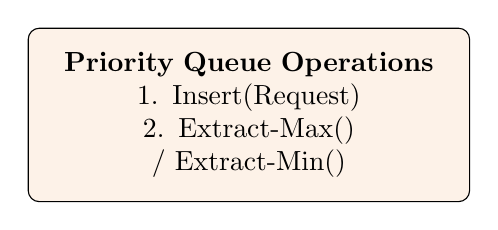
\begin{tikzpicture}
            \node[draw, rounded corners, fill=accent!10, text width=5cm, align=center, inner sep=2ex] (queue) at (0,0) {\textbf{Priority Queue Operations}\\1. Insert(Request)\\2. Extract-Max() / Extract-Min()};
        \end{tikzpicture}
    \end{center}
    \vspace{0.5cm}
    \begin{itemize}
        \item We need a data structure that always serves the highest priority item first, regardless of arrival time.
        \item This structure is called a \textbf{Priority Queue}.
    \end{itemize}
\end{frame}

\begin{frame}{Implementing a Priority Queue: Binary Heaps}
    \textbf{What is a Binary Heap?}
    \begin{itemize}
        \item A \textit{perfect} or \textit{almost complete} binary tree.
        \item It must satisfy the \textbf{Heap Property}.
        \item \textbf{Max-Heap:} Every parent is strictly $\ge$ its children.
        \item \textbf{Min-Heap:} Every parent is strictly $\le$ its children.
    \end{itemize}
\end{frame}

\begin{frame}{Visualizing a Binary Heap}
    \begin{center}
        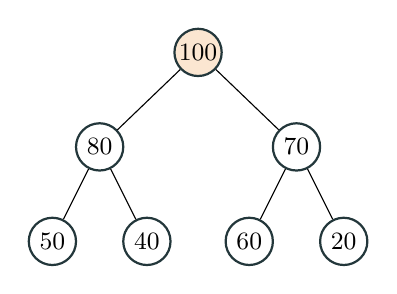
\begin{tikzpicture}[level distance=1.2cm,
          level 1/.style={sibling distance=2.5cm},
          level 2/.style={sibling distance=1.2cm}]
          \node[hnode, fill=accent!20] {100}
            child {node[hnode] {80}
              child {node[hnode] {50}}
              child {node[hnode] {40}}
            }
            child {node[hnode] {70}
              child {node[hnode] {60}}
              child {node[hnode] {20}}
            };
        \end{tikzpicture}
        
        \vspace{0.3cm}
        \small{\textit{A simple Max-Heap giving priority to the highest value.}}
    \end{center}
\end{frame}

\begin{frame}{Binary Heap Performance}
    Using a Binary Heap is very efficient for basic tasks!
    \vspace{0.3cm}
    \begin{itemize}
        \item \textbf{Add (Insert):} $\mathcal{O}(\log n)$ time.
        \item \textbf{Remove (Extract):} $\mathcal{O}(\log n)$ time.
    \end{itemize}
    \vspace{0.3cm}
    \textit{It perfectly serves our basic mailing system!}
\end{frame}

\begin{frame}{The Problem of Scale}
    \begin{alertblock}{Service Expansion}
        Our mailing service becomes wildly popular! We upgrade the servers to use \textbf{Multithreading}.
    \end{alertblock}
    \vspace{0.5cm}
    \begin{itemize}
        \item Each thread now handles a chunk of traffic and builds its own separate heap.
        \item When threads complete their chunk, their heaps must be \textbf{merged} into the unified master heap.
    \end{itemize}
\end{frame}

\begin{frame}{The Merging Bottleneck}
    \textbf{The problem with Binary Heaps:}
    \vspace{0.3cm}
    \begin{itemize}
        \item Merging two binary heaps is \textbf{extremely slow}.
        \item Adding elements one by one takes $\mathcal{O}(n \log n)$ time.
        \item Creating a brand new array and rebuilding from scratch takes $\mathcal{O}(n)$ time.
    \end{itemize}
    \vspace{0.5cm}
    \textit{Can we merge faster than $\mathcal{O}(n)$?}
\end{frame}

\begin{frame}{The Mathematical Analogy: Sticks}
    Imagine you are physically merging a pile of \textbf{25} sticks with \textbf{18} sticks.
    \vspace{0.5cm}
    \begin{itemize}
        \item If you add them one-by-one to the new pile, it takes you exactly \textbf{18 operations}.
        \item This is strictly linear time $\mathcal{O}(n)$.
        \item Is there a smarter way to group things?
    \end{itemize}
\end{frame}

\begin{frame}{The Binary Addition Analogy}
    Instead of counting by 1, consider grouping items in powers of two, just like binary numbers!
    \vspace{0.3cm}
    \begin{itemize}
        \item $25_{10} = \mathbf{11001_2}$
        \item $18_{10} = \mathbf{10010_2}$
        \item By adding bit-by-bit mathematically, it only takes $\approx \textbf{5 steps}$.
        \item Each "bit" represents a different magnitude of numbers! (1, 2, 4, 8...).
    \end{itemize}
    \vspace{0.3cm}
    \textbf{Logarithmic time $\mathcal{O}(\log n)$.}
\end{frame}

\begin{frame}{The Solution: Binomial Heaps}
    \begin{center}
        \textbf{What if our Data Structure mirrored the Binary Number System?}
    \end{center}
    \vspace{0.3cm}
    \begin{itemize}
        \item Instead of one monolithic tree, we use a \textbf{forest} (a collection) of structured trees.
        \item If our trees represented powers of 2, we could literally merge heaps by "adding bits".
        \item This is exactly what a \textbf{Binomial Heap} is!
    \end{itemize}
\end{frame}


% PART 2: Md. Sium (Structure & Merging)

\section{Part 2: Binomial Trees \& Merging\\ \small{(Presented by Md. Sium)}}

\begin{frame}{The Building Blocks: Powers of Two}
    A Binomial Heap is composed of special trees called \textbf{Binomial Trees} ($B_k$).
    \vspace{0.3cm}
    \begin{itemize}
        \item Every tree has exactly $2^k$ nodes.
        \item We build larger trees by simply snapping two smaller, identical trees together!
    \end{itemize}
\end{frame}

\begin{frame}{Constructing Binomial Trees: $B_0$ and $B_1$}
    \begin{itemize}
        \item A $B_0$ tree has $2^0 = 1$ node.
        \item A $B_1$ tree is made by making one $B_0$ tree the child of another's root. ($2^1 = 2$ nodes).
    \end{itemize}
    \vspace{0.5cm}
    \begin{center}
        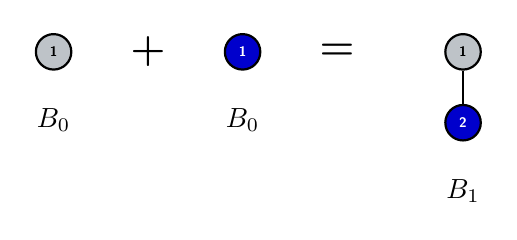
\begin{tikzpicture}[x=0.8cm, y=0.9cm]
            \treeBZero{0}{0}{bh}
            \node[below=0.6cm] at (0,0) {$B_0$};
            
            \node[font=\Large\bfseries] at (1.5,0) {+};
            
            \treeBZero{3}{0}{bhb}
            \node[below=0.6cm] at (3,0) {$B_0$};
            
            \node[font=\Large\bfseries] at (4.5,0) {=};
            
            \begin{scope}[shift={(6.5,0)}, every node/.style={bh}]
                \node (n1) at (0,0) {1}; \node[bhb] (n2) at (0,-1) {2}; \draw[lnk] (n1)--(n2);
            \end{scope}
            \node[below=1.5cm] at (6.5,0) {$B_1$};
        \end{tikzpicture}
    \end{center}
\end{frame}

\begin{frame}{Constructing Binomial Trees: $B_2$ and $B_3$}
    \begin{itemize}
        \item A $B_k$ tree is always created by joining a $B_{k-1}$ tree with another $B_{k-1}$ tree.
        \item \textit{Note: The smaller root value always stays on top to preserve the min-heap property!}
    \end{itemize}
    \vspace{0.2cm}
    \begin{center}
        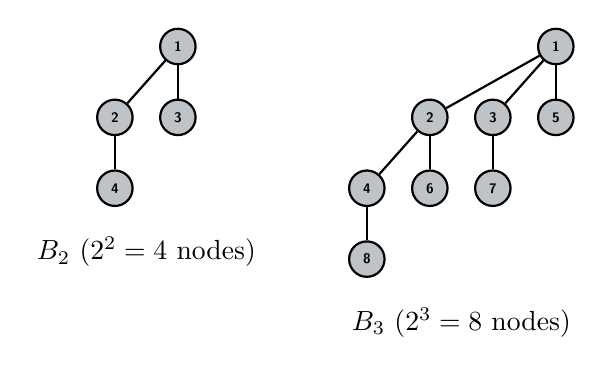
\begin{tikzpicture}[x=0.8cm, y=0.9cm]
            \treeBTwo{0}{0}{bh}
            \node[below=2.3cm] at (-0.5,0) {$B_2$ ($2^2=4$ nodes)};
            
            \treeBThree{6}{0}{bh}
            \node[below=3.2cm] at (4.5,0) {$B_3$ ($2^3=8$ nodes)};
        \end{tikzpicture}
    \end{center}
\end{frame}

\begin{frame}{The Structure of a Binomial Forest}
    \begin{itemize}
        \item Standard properties of a $B_k$ tree:
        \item It has depth exactly $k$.
        \item The root has exactly $k$ children.
        \item The children are roots of binomial trees of orders $k-1, k-2, \dots, 0$ ordered from left to right!
    \end{itemize}
\end{frame}

\begin{frame}{Anatomy of a Binomial Heap}
    \vspace{-0.2cm}
    \begin{center}
    \resizebox{0.9\textwidth}{!}{
    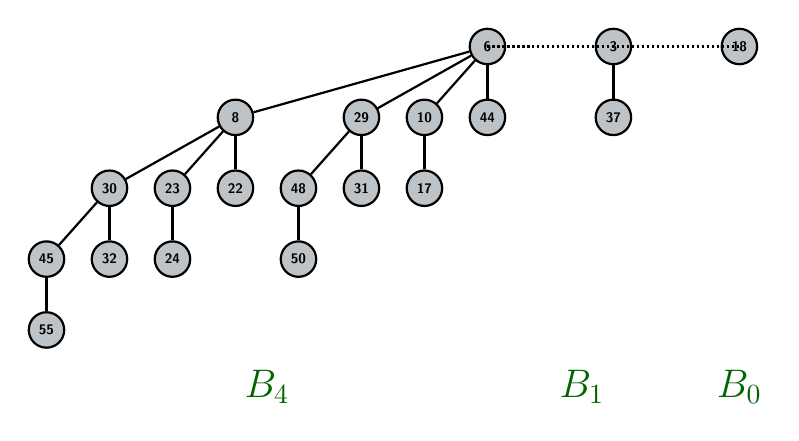
\begin{tikzpicture}[x=0.8cm, y=0.9cm]
        \treeSix{0}{0}{bh}
        \treeThree{2}{0}{bh}
        \treeEighteen{4}{0}{bh}
        \draw[dlnk] (0,0) -- (2,0) -- (4,0);

        \node[draw=none, fill=none, text=labelgreen, font=\Large\bfseries] at (-3.5, -4.8) {$B_4$};
        \node[draw=none, fill=none, text=labelgreen, font=\Large\bfseries] at (1.5, -4.8) {$B_1$};
        \node[draw=none, fill=none, text=labelgreen, font=\Large\bfseries] at (4, -4.8) {$B_0$};
    \end{tikzpicture}
    }
    \end{center}
\end{frame}

\begin{frame}{Representing Arbitrary numbers of nodes}
    If Binomial Trees must have exactly $2^k$ nodes, how do we store an odd number of requests?
    \vspace{0.4cm}
    \begin{itemize}
        \item Suppose our heap has exactly \textbf{13 nodes}.
        \item $13$ in binary is $\mathbf{1101_2}$.
        \item That breaks down to $13 = 8 + 4 + 1$.
        \item Therefore, our forest must be made up of exactly: $B_3, B_2, \text{and } B_0$.
    \end{itemize}
\end{frame}

\begin{frame}{The 13 Nodes Visualized}
    \begin{center}
        \resizebox{0.95\textwidth}{!}{
        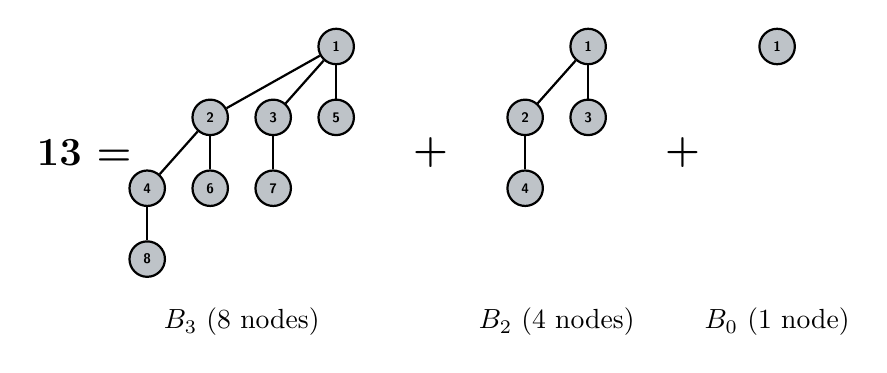
\begin{tikzpicture}[x=0.8cm, y=0.9cm]
            \node[font=\Large\bfseries] at (-2, -1.5) {13 = };
            
            \treeBThree{2}{0}{bh}
            \node[below=3.2cm] at (0.5,0) {$B_3$ (8 nodes)};
            
            \node[font=\Large\bfseries] at (3.5, -1.5) {+};
            
            \treeBTwo{6}{0}{bh}
            \node[below=3.2cm] at (5.5,0) {$B_2$ (4 nodes)};

            \node[font=\Large\bfseries] at (7.5, -1.5) {+};
            
            \treeBZero{9}{0}{bh}
            \node[below=3.2cm] at (9,0) {$B_0$ (1 node)};
        \end{tikzpicture}
        }
    \end{center}
\end{frame}

\begin{frame}{The 13 Nodes Visualized}
    \begin{center}
        \resizebox{0.95\textwidth}{!}{
        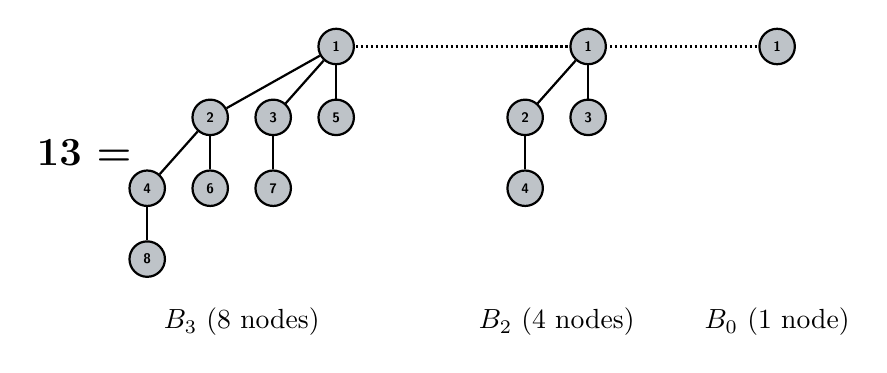
\begin{tikzpicture}[x=0.8cm, y=0.9cm]
            \draw[dlnk] (2,0) -- (6,0) -- (9,0);
            \node[font=\Large\bfseries] at (-2, -1.5) {13 = };
            
            \treeBThree{2}{0}{bh}
            \node[below=3.2cm] at (0.5,0) {$B_3$ (8 nodes)};
            
            % \draw[dlnk] (2,0) -- (8,0) -- (10,0);
            
            \treeBTwo{6}{0}{bh}
            \node[below=3.2cm] at (5.5,0) {$B_2$ (4 nodes)};

            
            
            \treeBZero{9}{0}{bh}
            \node[below=3.2cm] at (9,0) {$B_0$ (1 node)};
        \end{tikzpicture}
        }
    \end{center}
\end{frame}

\begin{frame}{Addition Example: 19 Nodes + 7 Nodes}
    \begin{center}
        What if we want to merge a heap containing exactly 7 nodes with a heap containing exactly 19 nodes?
        \vspace{0.4cm}
        \begin{itemize}
            \item $19$ in binary is $\mathbf{10011_2}$.
            \item That breaks down to $19 = 16 + 2 + 1$.
            \item The forest has the trees: $B_4, B_1, \text{and } B_0$.
        \end{itemize}
        \vspace{0.4cm}
        \begin{itemize}
            \item $7$ in binary is $\mathbf{0111_2}$.
            \item That breaks down to $7 = 4 + 2 + 1$.
            \item The forest has the trees: $B_2, B_1, \text{and } B_0$.
        \end{itemize}
    \end{center}
\end{frame}

\begin{frame}{Binomial Heap: Union (Initial State)}
    \vspace{-0.3cm}
    \begin{center}
    \resizebox{0.68\textwidth}{!}{
    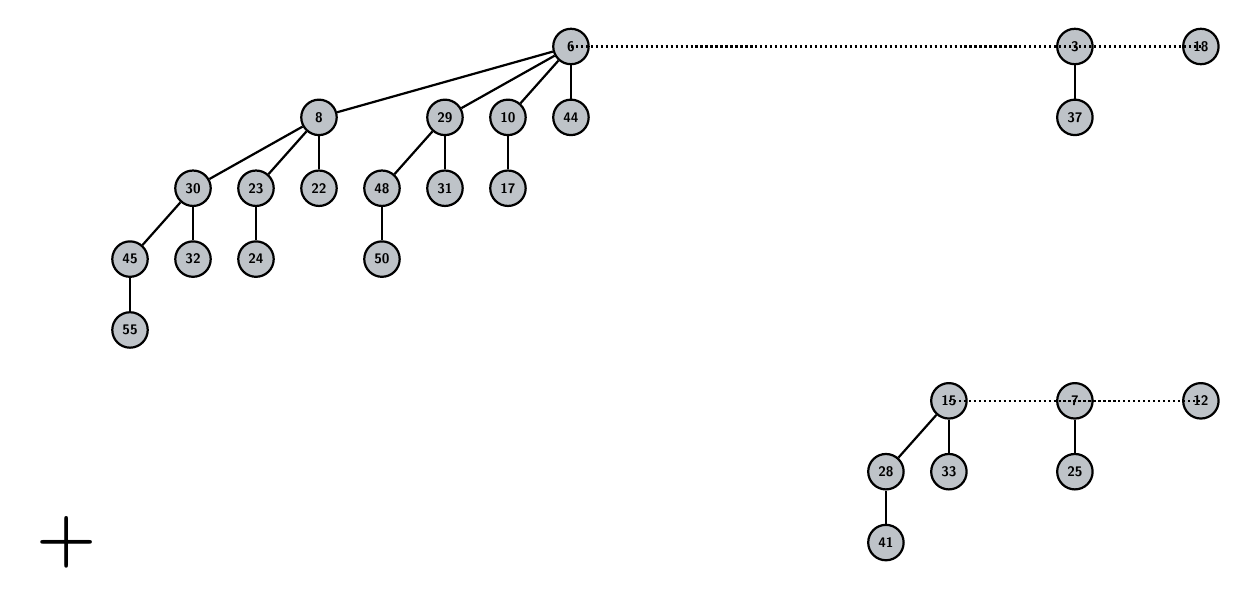
\begin{tikzpicture}[x=0.8cm, y=0.9cm]
        \treeSix{0}{0}{bh} \treeThree{8}{0}{bh} \treeEighteen{10}{0}{bh}
        \draw[dlnk] (0,0) -- (8,0) -- (10,0);
        
        \treeFifteen{6}{-5}{bh} \treeSeven{8}{-5}{bh} \treeTwelve{10}{-5}{bh}
        \draw[dlnk] (6,-5) -- (8,-5) -- (10,-5);
        
        \node[font=\Huge\bfseries] at (-8, -7) {+};
    \end{tikzpicture}
    }
    \end{center}
    \vfill
    \begin{flushleft}
        \scriptsize
        \renewcommand{\arraystretch}{0.9}
        \begin{tabular}{r c c c c c l}
             & $B_4$ & $B_3$ & $B_2$ & $B_1$ & $B_0$ & \\
          19 & 1 & 0 & 0 & 1 & 1 & ($10011_2$) \\
        +  7 & 0 & 0 & 1 & 1 & 1 & ($00111_2$) \\
        \hline
             &   &   &   &   &   & 
        \end{tabular}
    \end{flushleft}
\end{frame}

\begin{frame}{Binomial Heap: Union (Merge $B_0$)}
    \vspace{-0.3cm}
    \begin{center}
    \resizebox{0.55\textwidth}{!}{
    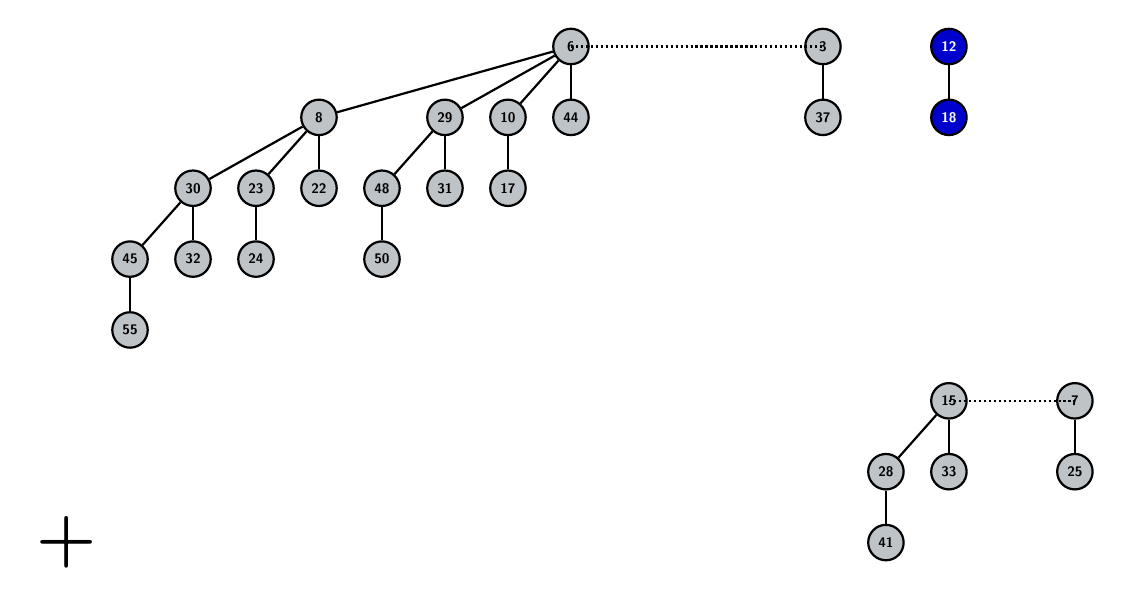
\begin{tikzpicture}[x=0.8cm, y=0.9cm]
        \treeSix{0}{0}{bh} \treeThree{4}{0}{bh}
        \draw[dlnk] (0,0) -- (4,0);
        
        \treeTwelveMerged{6}{0}{bhb}
        
        \treeFifteen{6}{-5}{bh} \treeSeven{8}{-5}{bh}
        \draw[dlnk] (6,-5) -- (8,-5);
        
        \node[font=\Huge\bfseries] at (-8, -7) {+};
    \end{tikzpicture}
    }
    \end{center}
    \vfill
    \begin{flushleft}
        \scriptsize
        \renewcommand{\arraystretch}{0.9}
        \begin{tabular}{r c c c c c}
             & $B_4$ & $B_3$ & $B_2$ & $B_1$ & \color{blue}$B_0$ \\
          19 & 1 & 0 & 0 & 1 & \textbf{1} \\
        +  7 & 0 & 0 & 1 & 1 & \textbf{1} \\
        \hline
        Carry&   &   &   & \color{blue}1 & \\
      Result &   &   &   &   & \color{red}\textbf{0}
        \end{tabular}
    \end{flushleft}
\end{frame}

\begin{frame}{Binomial Heap: Union (Merge $B_1$)}
    \vspace{-0.3cm}
    \begin{center}
    \resizebox{0.55\textwidth}{!}{
    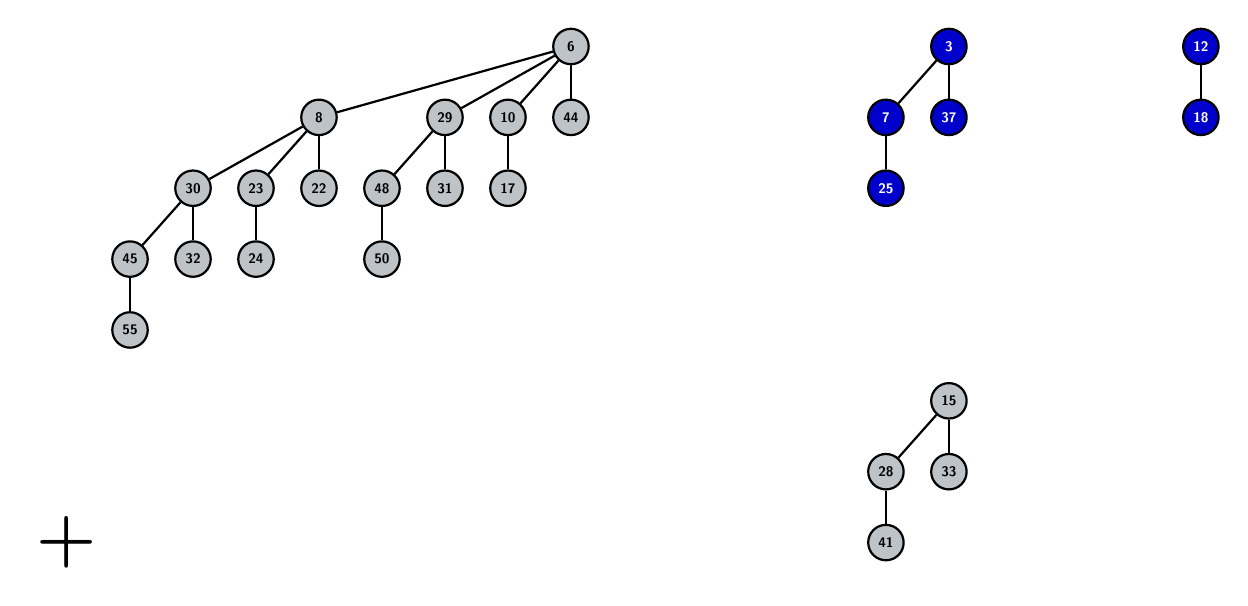
\begin{tikzpicture}[x=0.8cm, y=0.9cm]
        \treeSix{0}{0}{bh}
        
        \treeThreeMerged{6}{0}{bhb}
        \treeTwelveMerged{10}{0}{bhb}
        
        \treeFifteen{6}{-5}{bh}
        
        \node[font=\Huge\bfseries] at (-8, -7) {+};
    \end{tikzpicture}
    }
    \end{center}
    \vfill
    \begin{flushleft}
        \scriptsize
        \renewcommand{\arraystretch}{0.9}
        \begin{tabular}{r c c c c c}
             & $B_4$ & $B_3$ & $B_2$ & \color{blue}$B_1$ & $B_0$ \\
          19 & 1 & 0 & 0 & \textbf{1} & 1 \\
        +  7 & 0 & 0 & 1 & \textbf{1} & 1 \\
        \hline
        Carry&   &   & \color{blue}1 & \textbf{1} & \\
      Result &   &   &   & \color{red}\textbf{1} & 0
        \end{tabular}
    \end{flushleft}
\end{frame}

\begin{frame}{Binomial Heap: Union (Merge $B_2$)}
    \vspace{-0.3cm}
    \begin{center}
    \resizebox{0.68\textwidth}{!}{
    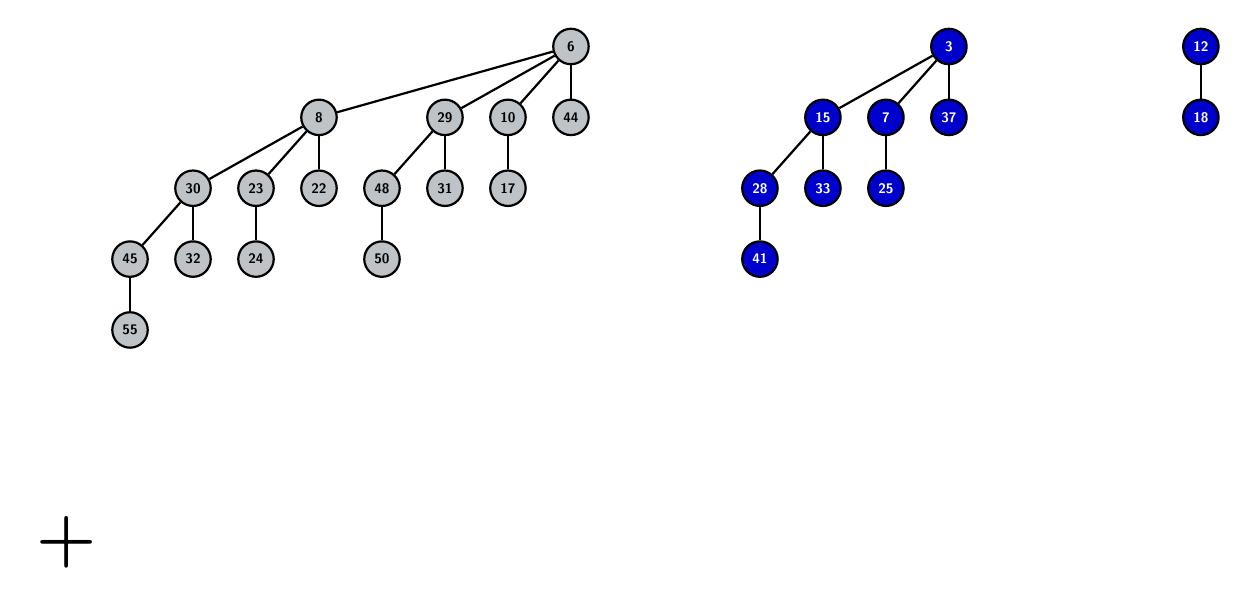
\begin{tikzpicture}[x=0.8cm, y=0.9cm]
        \treeSix{0}{0}{bh}
        
        \treeThreeFinal{6}{0}{bhb}
        \treeTwelveMerged{10}{0}{bhb}
        
        \node[font=\Huge\bfseries] at (-8, -7) {+};
    \end{tikzpicture}
    }
    \end{center}
    \vfill
    \begin{flushleft}
        \scriptsize
        \renewcommand{\arraystretch}{0.9}
        \begin{tabular}{r c c c c c}
             & $B_4$ & $B_3$ & \color{blue}$B_2$ & $B_1$ & $B_0$ \\
          19 & 1 & 0 & \textbf{0} & 1 & 1 \\
        +  7 & 0 & 0 & \textbf{1} & 1 & 1 \\
        \hline
        Carry&   & \color{blue}1 & \textbf{1} & 1 & \\
      Result &   &   & \color{red}\textbf{0} & 1 & 0
        \end{tabular}
    \end{flushleft}
\end{frame}

\begin{frame}{Binomial Heap: Union (Final Result)}
    \vspace{-0.3cm}
    \begin{center}
    \resizebox{0.68\textwidth}{!}{
    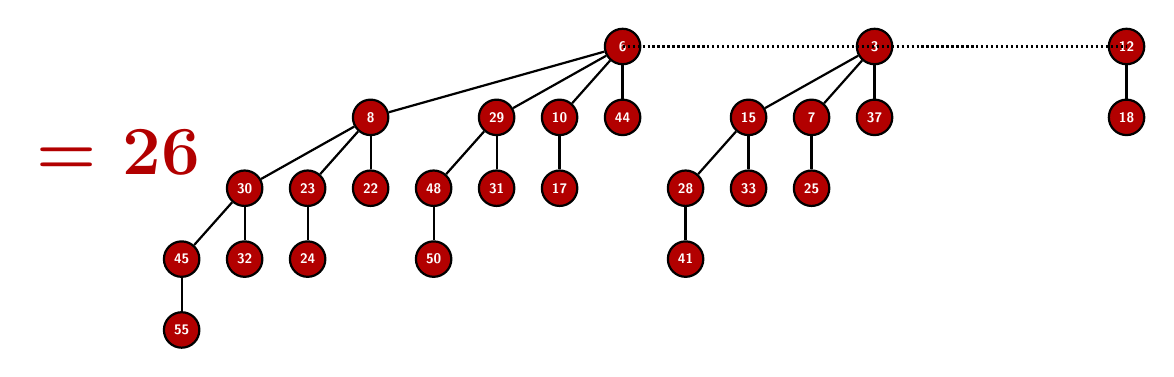
\begin{tikzpicture}[x=0.8cm, y=0.9cm]
        \treeSix{0}{0}{bhr}
        \treeThreeFinal{4}{0}{bhr}
        \treeTwelveMerged{8}{0}{bhr}
        
        \draw[dlnk] (0,0) -- (4,0) -- (8,0);
        
        \node[font=\Huge\bfseries, text=red!70!black] at (-8, -1.5) {= 26};
    \end{tikzpicture}
    }
    \end{center}
    \vfill
    \begin{flushleft}
        \scriptsize
        \renewcommand{\arraystretch}{0.9}
        \begin{tabular}{r c c c c c l}
             & $B_4$ & $B_3$ & $B_2$ & $B_1$ & $B_0$ & \\
          19 & 1 & 0 & 0 & 1 & 1 & ($10011_2$) \\
        +  7 & 0 & 0 & 1 & 1 & 1 & ($00111_2$) \\
        \hline
      Result & \color{red}\textbf{1} & \color{red}\textbf{1} & \color{red}\textbf{0} & \color{red}\textbf{1} & \color{red}\textbf{0} & ($11010_2 = \textbf{26}$)
        \end{tabular}
    \end{flushleft}
\end{frame}

\begin{frame}{What if there ARE Carries?}
    Let's look at merging two trees of the \textbf{same order}.
    \vspace{0.2cm}
    \begin{center}
    \resizebox{0.65\textwidth}{!}{
    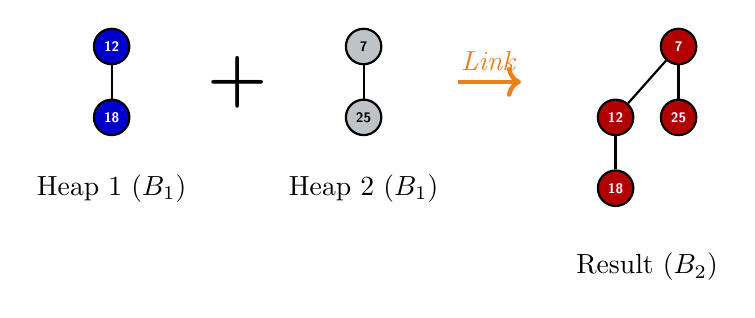
\begin{tikzpicture}[x=0.8cm, y=0.9cm]
        \begin{scope}[shift={(0,0)}, every node/.style={bhb}]
            \node (n12) at (0,0) {12}; \node (n18) at (0,-1) {18}; \draw[lnk] (n12)--(n18);
        \end{scope}
        \node[below=1.5cm] at (0,0) {Heap 1 ($B_1$)};

        \node[font=\Huge\bfseries] at (2, -0.5) {+};

        \begin{scope}[shift={(4,0)}, every node/.style={bh}]
            \node (n7) at (0,0) {7}; \node (n25) at (0,-1) {25}; \draw[lnk] (n7)--(n25);
        \end{scope}
        \node[below=1.5cm] at (4,0) {Heap 2 ($B_1$)};
        
        \draw[->, ultra thick, accent] (5.5, -0.5) -- (6.5, -0.5) node[midway, above] {\textit{Link}};

        \begin{scope}[shift={(9,0)}, every node/.style={bhr}]
            \node (n7) at (0,0) {7}; \node (n25) at (0,-1) {25};
            \node (n12) at (-1,-1) {12}; \node (n18) at (-1,-2) {18};
            \draw[lnk] (n7)--(n25); \draw[lnk] (n7)--(n12); \draw[lnk] (n12)--(n18);
        \end{scope}
        \node[below=2.5cm] at (8.5,0) {Result ($B_2$)};
        
    \end{tikzpicture}
    }
    \end{center}
    \vspace{0.2cm}
    \begin{itemize}
        \item We compare the roots: $7 < 12$.
        \item The $12$ (and its subtree) becomes the leftmost child of the $7$.
        \item $B_1 + B_1 = \text{Carry } B_2$!
    \end{itemize}
\end{frame}

\begin{frame}{Merging: Summarized with Carries}
    If a collision occurs ($1 + 1$ in binary):
    \vspace{0.3cm}
    \begin{itemize}
        \item Keep the smaller root.
        \item Make the larger root its leftmost child.
        \item The order of the tree increases by 1 (We carry the bit to the left!).
        \item We repeat this step until there are no remaining duplicate tree orders.
    \end{itemize}
    \vspace{0.5cm}
    \begin{alertblock}{The Magic of Binomial Merging}
        Because we only traverse up to $\log n$ trees, a full merge operation takes at most \textbf{$\mathcal{O}(\log n)$} steps. A massive upgrade over $O(n)$!
    \end{alertblock}
\end{frame}


% PART 3: Md. Fuad Al Alam (Operations & Complexity)
\section{Part 3: Operations \& Complexity\\ \small{(Presented by Md. Fuad Al Alam)}}

\begin{frame}{The Power of Merge}
    \textbf{The golden rule of Binomial Heaps:}
    \vspace{0.3cm}
    \begin{itemize}
        \item The entire data structure revolves around the $O(\log n)$ \textit{Merge} operation!
        \item For nearly every major operation aside from finding a node, we just configure the data slightly, and then forcefully call \textit{Merge} to handle the heavy lifting.
    \end{itemize}
\end{frame}

\begin{frame}{Operation: Find Minimum}
    \begin{itemize}
        \item The smallest value in any $B_k$ tree is strictly its root node.
        \item Therefore, the smallest value in the entire forest MUST be one of the root nodes.
        \item Since there are at most $\log n$ trees, we only need to scan the linked list of roots!
    \end{itemize}
\end{frame}

\begin{frame}{Find Minimum: Complexity Analysis}
    \begin{itemize}
        \item Scanning a linked list of size $\log n$ takes $\mathbf{\mathcal{O}(\log n)}$.
        \item \textbf{Optimization:} We usually keep an external pointer directly targeting the global minimum root.
        \item By updating this pointer during merges and extractions, \textit{Find Minimum} becomes a true $\mathbf{\mathcal{O}(1)}$ operation.
    \end{itemize}
\end{frame}

\begin{frame}{Operation: Add (Insert)}
    \begin{itemize}
        \item Adding a singular request to our mailing priority queue is surprisingly simple!
        \item We treat the new element not as a standalone item, but as a \textit{brand new Binomial Heap} containing exactly one node ($B_0$).
    \end{itemize}
\end{frame}

\begin{frame}{Operation: Add (Visualizing Insertion)}
    \begin{center}
        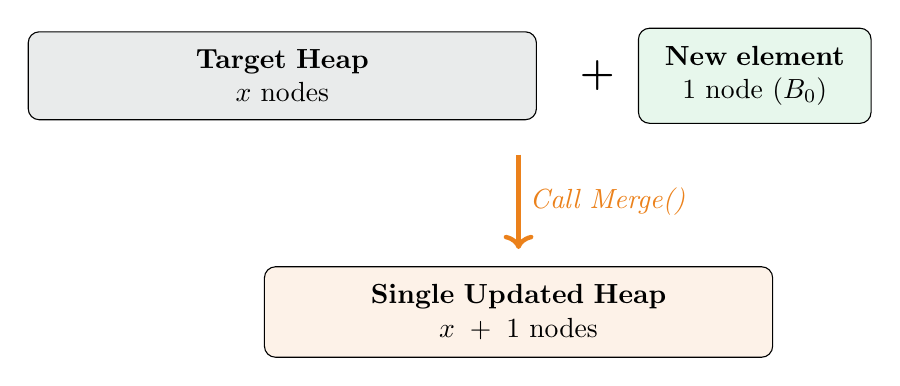
\begin{tikzpicture}
            \node[draw, rounded corners, fill=primary!10, text width=6cm, align=center, inner sep=1.5ex] (mergeNode) at (0,0) {\textbf{Target Heap}\\$x$ nodes};
            \node[font=\Large\bfseries] at (4,0) {+};
            \node[draw, rounded corners, fill=success!10, text width=2.5cm, align=center, inner sep=1.5ex] (b0Node) at (6,0) {\textbf{New element}\\1 node ($B_0$)};
            
            \draw[->, ultra thick, accent] (3, -1) -- (3, -2.2) node[midway, right] {\textit{Call Merge()}};
            \node[draw, rounded corners, fill=accent!10, text width=6cm, align=center, inner sep=1.5ex] (resultNode) at (3,-3) {\textbf{Single Updated Heap}\\$x+1$ nodes};
        \end{tikzpicture}
    \end{center}
    \vspace{0.3cm}
    \textbf{Time Complexity:} Because $Merge$ runs in $O(\log n)$ time, our $Add$ operation naturally runs in bounded $\mathbf{\mathcal{O}(\log n)}$ time!
\end{frame}

\begin{frame}{Operation: Decrease Key}
    \begin{itemize}
        \item Sometimes a premium subscriber upgrades their VIP tier, and their queue priority strictly decreases (gets closer to priority index 0!).
        \item We adjust the node's value.
        \item But wait, making a value smaller might violate the min-heap property of its tree!
    \end{itemize}
\end{frame}

\begin{frame}{Operation: Decrease Key (Bubbling)}
    \begin{itemize}
        \item We push the decreased value upward toward the root, swapping with its parent until the heap property is restored.
        \item This is affectionately known as \textit{"Bubbling up"}.
        \item Because the absolute maximum depth of a tree containing $n$ elements is $\log n$, we can bubble up at most $\log n$ times!
        \item \textbf{Time Complexity: $\mathbf{\mathcal{O}(\log n)}$}
    \end{itemize}
\end{frame}

\begin{frame}{Operation: Extract Minimum}
    \begin{itemize}
        \item To process and remove the highest priority mail, we must extract the global minimum.
        \item Step 1: Remove the minimum root from the linked list of roots.
        \item Step 2: What happens to its orphaned children?
    \end{itemize}
\end{frame}

\begin{frame}{Operation: Extract Minimum (Merging back)}
    \begin{alertblock}{The magic of the Binomial Tree}
        If you delete the root of a $B_k$ tree, its remaining children are exactly the trees $B_{k-1}, B_{k-2}, \dots B_0$.
    \end{alertblock}
    \vspace{0.5cm}
    \begin{itemize}
        \item The orphaned children literally form a perfectly valid, standalone Binomial forest!
        \item We treat the children as a second heap, and call $Merge()$ to fuse it back into the main forest.
        \item \textbf{Time Complexity: $\mathbf{\mathcal{O}(\log n)}$}
    \end{itemize}
\end{frame}

\begin{frame}{Complexity Summary: The Binomial Advantage}
    \begin{center}
        \large \textit{Everything piggybacks on the efficient Merge!}
        
        \vspace{0.1cm}
        \renewcommand{\arraystretch}{1.3}
        \begin{tabular}{lc}
            \toprule
            \textbf{Operation} & \textbf{Binomial Heap} \\
            \midrule
            Find Minimum   & $\mathcal{O}(1)$ \small{\textit{(with pointer)}} \\
            Insert Node    & $\mathcal{O}(\log n)$ \\
            Decrease Key   & $\mathcal{O}(\log n)$ \\
            \textbf{Merge Heaps}    & \textbf{$\mathcal{O}(\log n)$} \quad $\leftarrow \text{The Engine!}$ \\
            Extract Minimum& $\mathcal{O}(\log n)$ \\
            \bottomrule
        \end{tabular}
    \end{center}
\end{frame}

\begin{frame}{Comparison: Binary vs. Binomial Heaps}
    \begin{center}
        \renewcommand{\arraystretch}{1.3}
        \begin{tabular}{lcc}
            \toprule
            \textbf{Operation} & \textbf{Binary Heap} & \textbf{Binomial Heap} \\
            \midrule
            Find Min   & $\mathcal{O}(1)$ & $\mathcal{O}(1)$ \\
            Insert     & $\mathcal{O}(\log n)$ & $\mathcal{O}(\log n)$ \\
            Extract Min& $\mathcal{O}(\log n)$ & $\mathcal{O}(\log n)$ \\
            \rowcolor{accent!20}
            \textbf{Merge}      & $\mathcal{O}(n)$ & $\mathbf{\mathcal{O}(\log n)}$ \\
            \bottomrule
        \end{tabular}
    \end{center}
    
    \vspace{0.2cm}
    \textbf{Takeaway:} For multithreaded or distributed systems where heaps must coalesce, Binomial Heaps reign supreme.
\end{frame}

\begin{frame}{The Theoretical Ideal: Fibonacci Heaps}
    Could we push the limits even further? Yes, using \textbf{Fibonacci Heaps}.
    \vspace{0.3cm}
    \begin{itemize}
        \item Employs severe \textit{"lazy evaluation"}.
        \item It simply throws trees together in $O(1)$ time and delays actually merging them until an \textit{Extract} call absolutely forces it to do the work.
        \item Achieves an unheard of \textbf{$\mathcal{O}(1)$ amortized time} for Insert, Merge, and Decrease Key!
    \end{itemize}
\end{frame}

\begin{frame}{The Catch: Why Binomial wins in Practice}
    \begin{itemize}
        \item While Fibonacci Heaps are mathematically beautiful and give Dijkstra's algorithm its theoretical fastest bounds...
        \item They suffer from immense \textbf{constant overhead factors}.
        \item They rely heavily on pointers, causing massive CPU cache misses.
        \item Their implementation is exceptionally complex and prone to errors.
    \end{itemize}
    \vspace*{-0.2cm}
    \begin{alertblock}{Conclusion}
        Binomial Heaps strike the perfect, practical balance between optimal merge performance and sensible engineering complexity.
    \end{alertblock}
\end{frame}

\begin{frame}[standout]
    Thank You! \\
\end{frame}

\end{document}
